In order to investigate the characteristics of particles, it is necessary to rely on particle detectors. Charged particles interact with other particles primarily via Coulomb scattering and are the easiest to detect because of it. Some detectors are designed to measure the ionization produced by charged particles as they pass through a medium \cite{IntroToNuclearAndParticle}. When it comes to neutrons, the detection becomes more complicated. Neutrons do not produce any ionization nor undergo Coulomb scattering. Instead, they interact with the target nucleus via nuclear reactions.

One way to detect neutrons is to cause them to react via nuclear interaction with a material, and then measure the ionization of the medium that the product (charged) particles induce. This is a common design for the so called ionization chambers, the detection device that concerns this work. The neutrons produced from the initial reaction with the target cannot be measured directly for the reason stated previously. Instead, they need to interact again and generate measurable charged particles. Further details will be exposed about ionization chambers in the next subsection. 

\subsection{Ionization Chambers}

Ionization chambers are a detector used in dosimetry to measure the dose delivered by a source of radiation \cite{RadiationOncologyInPhysicsHandbook}. Ionization chambers are a type of gas-filled detector, which is a device that is able to operate at different voltages according to the sensibility of the measurements it is intended to obtain. A gas-filled detector behaves as a ionization chamber at relatively low voltages \cite{IntroToNuclearAndParticle}. Regarding the design, a ionization chambers is a generally cylindrical cavity filled with a gas and contains an electrode placed in the center in the longitudinal direction. The cavity is surrounded by a conductive wall \cite{RadiationOncologyInPhysicsHandbook}. A commonly used chamber for radiation therapy dosimetry measurements is the 30010 Farmer \cite{PTWFarmer}. The basic design of a Farmer chamber is shown in Figure \ref{fig:Basic design of a Farmer ionization chamber}.



\begin{figure}[!h]
    \centering
    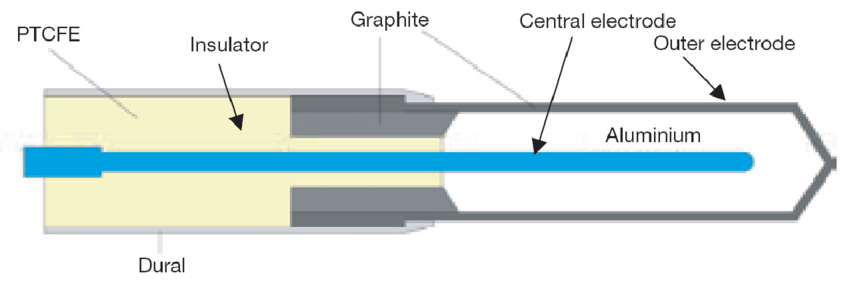
\includegraphics[scale = 0.35]{Master Thesis Manuel Galdon/figures/Basic-design-of-a-cylindrical-Farmer-type-ionisation-chamber-From-Podgorsak-2005a.png}
    \caption{Basic design of a Farmer Ionization Chamber.}
    \label{fig:Basic design of a Farmer ionization chamber}
\end{figure}

In Figure \ref{fig:Basic design of a Farmer ionization chamber}, all the constituent parts of the Farmer are pointed out. The PTCFE is polytrichloro-fluoroethylene \cite{DesignOfThimbleChamber}, an insulator material meant to reduce the leakage current \cite{RadiationOncologyInPhysicsHandbook}. A graphite sleeve is inserted to eliminate the disturbance caused by the remaining charges on the insulator \cite{DesignOfThimbleChamber}. The wall material is generally made of a low Z material to reduce the energy loss. The chamber is covered with a "cap", referred to as "dural" in Figure \ref{fig:Basic design of a Farmer ionization chamber} for calibration purposes. 

Incoming neutrons generated by a radiation source come into the sensitive region or gas-filled region of chamber and generate charged particles, including electrons and heavy ions. Applying a voltage to the electrode causes the charged particles to be attracted to it and, therefore, an increase in the total charge accumulated in the detector. This is the variable that can be measured to calibrate the device to finally calculate the total dose absorbed by the gas of the chamber.

Ionization chambers are able to provide high resolution measurements in terms of energy because there is no signal amplification. This means that the response of the chamber will be linear, and is due to the voltage that is applied to the electrode. A higher voltage would cause a strong amplification or even an avalanche effect in the charges present in the environment within the sensitive region \cite{IntroToNuclearAndParticle}.